\chapter{Deadlock}
Il deadlock è un blocco permanente di un insieme di processi, che o competono per delle risorse di sistema o comunicano tra loro. Il motivo di base per la nascita di un deadlock è la richiesta contemporanea delle stesse risorse da parte di due o più processi.

Le situazioni di deadlock possono essere raffigurate con un \textit{Joint Progess Diagram} come in Figura \ref{fig:jpd}. 

\begin{figure}[h]
    \centering
    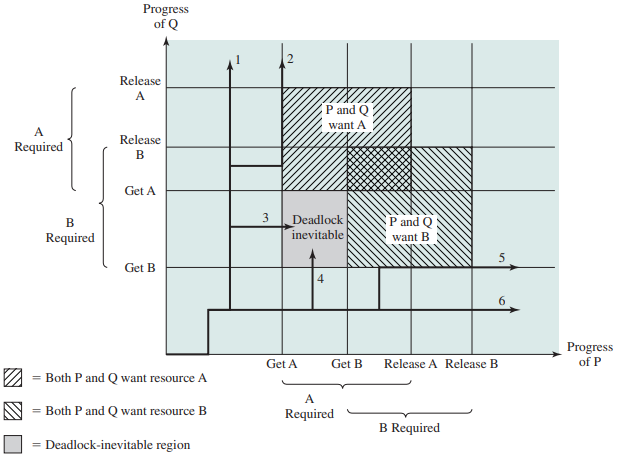
\includegraphics[width=0.49\linewidth]{images/jpd.PNG}
    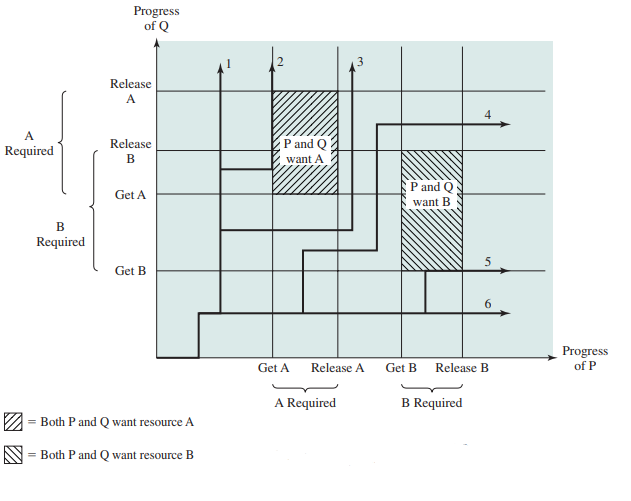
\includegraphics[width=0.49\linewidth]{images/jpd1.PNG}
    \caption{Joint Progress Diagram}
    \label{fig:jpd}
\end{figure}

Nel primo diagramma, nel momento in qui i processi \verb|P| e \verb|Q| chiedono una risorsa, prima di rilasciarla ne richiedono un'altra. Se il dispatcher manda in esecuzione \verb|P| e \verb|Q| prima di rilasciare le risorse si avrà sicuramente deadlock.

Nel secondo diagramma il processo \verb|P| richiede una risorsa e la rilascia prima di chiederne un'altra. In questo modo non potrà mai verificarsi il deadlock.

\section{Risorse}
Facciamo una distinzione tra le risorse utilizzate dai processi perché cambiano la definizione di deadlock.

\subsection*{Risorse riusabili}
Le risorse riusabili (\textit{reusable resources}) sono usabili da un solo processo alla volta e non vengono consumate (ad esempio processori, I/O channels, memoria primaria e secondaria, dispositivi, file, database, semafori). Una volta che un processo ottiene una risorsa riusabile, prima o poi la rilascia cosicché altri processi possano usarla a loro volta. Lo stallo può esistere solo se un processo ha una risorsa e ne richiede un'altra.

\begin{Example}{Deadlock con risorse riusabili}{}
    \textit{Supponiamo di avere due processi P e Q che richiedono e rilasciano le risorse D e T.}
    
    \begin{minipage}{\textwidth}
        \centering
        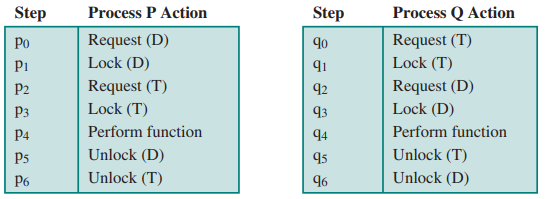
\includegraphics[width=0.6\linewidth]{images/esempio-deadlock.PNG}
        %\captionof{figure}{Esempio di semaforo}
    \end{minipage}

    Notiamo che se il dispatcher esegue \verb|P| fino a $p_1$ e poi passa a \verb|Q| otteniamo un deadlock perché le risorse \verb|T| in \verb|P| e \verb|D| in \verb|Q| non possono essere più richieste.
\end{Example}

\begin{Example}{Deadlock con risorse riusabili}{}
    \textit{Supponiamo che ci siano 200 KB di memoria disponibili, e che ci sia la seguente sequenza di richieste:}
    
    \begin{minipage}{\textwidth}
        \centering
        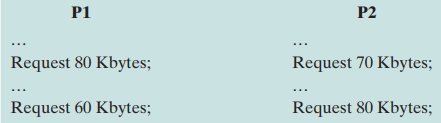
\includegraphics[width=0.6\linewidth]{images/esempio-deadlock1.PNG}
        %\captionof{figure}{Esempio di semaforo}
    \end{minipage}

    Notiamo che se il dispatcher esegue la prima richiesta di \verb|P|$_1$ e poi passa a \verb|P|$_2$ otteniamo un deadlock quando uno dei processi farà la seconda richiesta, perché in tutte e due i casi si supera lo spazio di memoria disponibile.
\end{Example}

\subsection*{Risorse consumabili}
Le risorse consumabili (\textit{comsumable resources}) vengono create (prodotte) e distrutte (consumate) (ad esempio interruzioni, segnali, messaggi, informazione nei buffer di I/O). Il deadlock viene generato se si fa una richiesta (bloccante) di una risorsa ancora non creata, ad esempio, un deadlock può avvenire su una ricezione bloccante.

\begin{Example}{Deadlock con risorse consumabili}{}
    \textit{Supponiamo che i processi facciano le seguenti richieste:}
    
    \begin{minipage}{\textwidth}
        \centering
        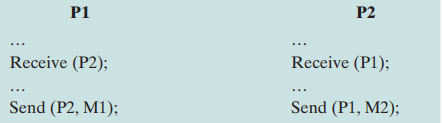
\includegraphics[width=0.6\linewidth]{images/esempio-deadlock2.PNG}
        %\captionof{figure}{Esempio di semaforo}
    \end{minipage}

    Nel momento in cui il dispatcher esegue la prima richiesta di \verb|P|$_1$ e poi passa a \verb|P|$_2$ otteniamo un deadlock perché non potrà essere esaudita né la \verb|Send| di \verb|P|$_1$ che quella di \verb|P|$_2$.
\end{Example}

\subsection*{Grafo dell'allocazione delle risorse}
Il grafo dell'allocazione delle risorse è un grafo diretto che rappresenta lo stato di processi e risorse rappresentati rispettivamente come nodi tondi e quadrati. Con le risorse riusabili si indica con una freccia (a) per la richiesta e al contrario (b) quando la richiesta è accordata (\textit{held}) (vedi Figura \ref{fig:grafo-allocazione}); mentre per le risorse consumabili non esiste l'Held e i pallini compaiono e scompaiono. 

Le condizioni per il deadlock con le risorse riusabili/consumabili sono:
\begin{itemize}
    \item \textit{Mutua esclusione}: quando un solo processo alla volta può usare una data risorsa;
    \item Richiesta di una risorsa quando se ne ha già una (\textit{hold-and-wait}): quando un processo può richiedere risorse mentre ne ha già bloccate altre/si può richiedere in modo bloccante una risorsa quando ancora non è stata creata;
    \item \textit{Mancanza di preemption} per le risorse: quando non si può sottrarre una risorsa ad un processo senza che quest'ultimo al rilasci;
    \item \textit{Attesa circolare}: quando esiste una catena chiusa di processi, in cui ciascun processo detiene una risorsa che è richiesta (invano) dal processo che lo segue nella catena/quando esiste una catena chiusa di processi, in cui ciascun processo dovrebbe creare una risorsa che è richiesta (invano) dal processo che lo segue nella catena.
\end{itemize}

\begin{figure}[h]
    \centering
    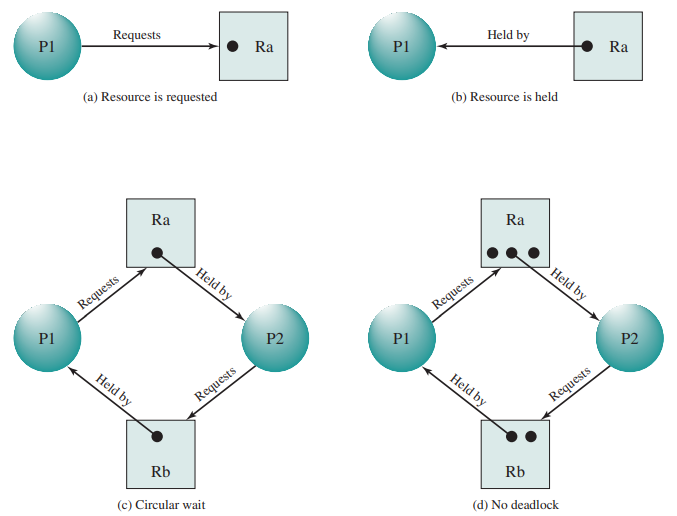
\includegraphics[width=0.6\linewidth]{images/grafo-allocazione.PNG}
    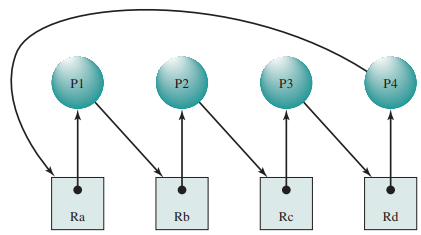
\includegraphics[width=0.39\linewidth]{images/grafo-allocazione1.PNG}
    \caption{Grafi dell'allocazione delle risorse}
    \label{fig:grafo-allocazione}
\end{figure}

L'esistenza vera e propria del deadlock si ha quando alle tre condizioni: mutua esclusione, richiesta di una risorsa quando se ne ha già una (\textit{hold-and-wait}) e mancanza di preemption per le risorse (che dipendono dalla stuttura del sistema operativo) si aggiunge l'attesa circolare.

\section{Prevenzione del deadlock}
Per prevenire il deadlock si cerca di far sì che una delle quattro condizioni sia sempre falsa. Ma non c'è modo per evitare la mutua esclusione, per l'hold-and-wait si impone ad un processo di richiedere tutte le sue risorse in una volta, per la mancanza di preemption per le risorse il sistema operativo può richiedere ad un processo di rilasciare le sue risorse e per l'attesa circolare si definisce un ordinamento crescente delle risorse, ovvero una risorsa viene data solo se segue quelle che il processo già detiene.

\section{Evitare il deadlock}
Per evitare il deadlock occorre decidere se l'attuale richiesta di una risorsa può portare ad un deadlock, se esaudita. Questo richiede la conoscenza delle richieste future e ci sono due possibilità: o non mandare in esecuzione un processo se le sue richieste possono portare a deadlock oppure non concedere una risorsa ad un processo se allocarla può portare a deadlock (algoritmo del banchiere).

\subsection*{Algoritmo del banchiere}
L'algoritmo del banchiere è valido per le risorse riusabili e fa si che il sistema proceda da uno stato non sicuro (\textit{unsafe} - il cammino porta a un deadlock) ad uno sicuro (\textit{safe} - il cammino non porta a un deadlock).

Le strutture dati utilizzate per questo algoritmo sono in Figura \ref{fig:strutture-dati-banchiere}.

\begin{figure}[h]
    \centering
    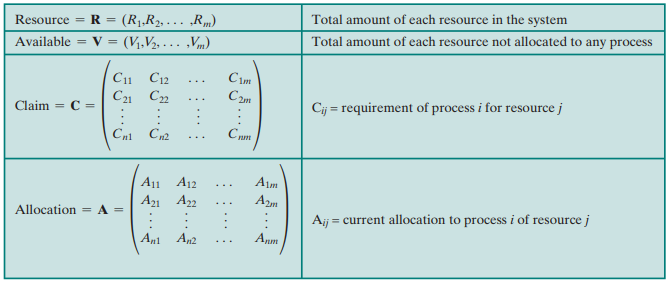
\includegraphics[width=0.8\linewidth]{images/strutture-dati-banchiere.PNG}
    \caption{Strutture dati dell'algoritmo del banchiere}
    \label{fig:strutture-dati-banchiere}
\end{figure}

\begin{Example}{Stato sicuro}{}
    \textit{Il seguente stato è sicuro perché esiste almeno un cammino che non porta a un deadlock:}
    
    \begin{minipage}{\textwidth}
        \centering
        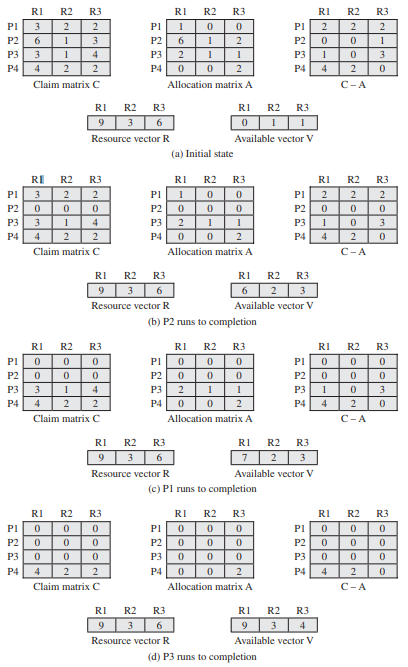
\includegraphics[width=0.6\linewidth]{images/stato-sicuro.PNG}
        %\captionof{figure}{Esempio di semaforo}
    \end{minipage}
\end{Example}

\begin{Example}{Stato non sicuro}{}
    \textit{Il seguente stato non è sicuro perché nessuno dei quattro processi può essere selezionato per andare in esecuzione:}
    
    \begin{minipage}{\textwidth}
        \centering
        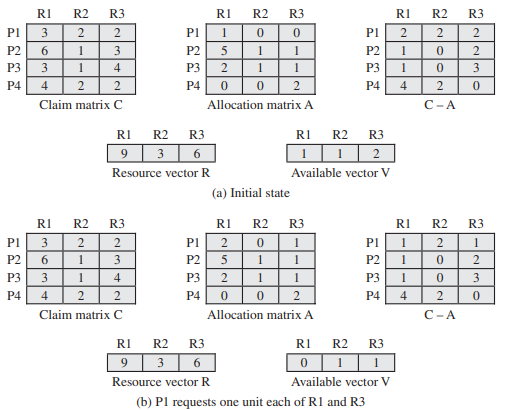
\includegraphics[width=0.6\linewidth]{images/stato-non-sicuro.PNG}
        %\captionof{figure}{Esempio di semaforo}
    \end{minipage}
\end{Example}

Lo pseudocodice dell'algoritmo è il seguente:
\begin{lstlisting}[language=C]
    /* Global data structures */
    struct state {
        int resource[m];
        int available[m];
        int claim[n][m];
        int alloc[n][m];
    }

    /* Resource alloc algorithm */
    if (alloc [i,*] + request [*] > claim [i,*])
        <error>; /* total request > claim*/
    else if (request [*] > available [*])
        <suspend process>;
    else { /* simulate alloc */
        <define newstate by:
        alloc [i,*] = alloc [i,*] + request [*];
        available [*] = available [*] - request [*]>;
    }
    if (safe (newstate))
        <carry out allocation>;
    else {
        <restore original state>;
        <suspend process>;
    }

    /*  Test for safety algorithm */
    boolean safe (state S) {
        int currentavail[m];
        process rest[<number of processes>];
        currentavail = available;
        rest = {all processes};
        possible = true;
        while (possible) {
            <find a process Pk in rest such that
            claim [k,*] - alloc [k,*]<= currentavail;
            if (found) { /* simulate execution of Pk */
                currentavail = currentavail + alloc [k,*];
                rest = rest - {Pk};
            }
            else possible = false;
        }
        return (rest == null);
    }
\end{lstlisting}

Con questo algoritmo occorre dichiarare il massimo uso di risorse; i processi devono essere indipendenti senza requisiti di sincronizzazione ovvero, devono essere liberi di andare in esecuzione in un qualsiasi ordine, altrimenti, non si può simularne l'esecuzione fino al completamento; ci deve essere un numero fissato di risorse da allocare; nessun processo deve terminare senza rilasciare le sue risorse.

\section{Rilevare il deadlock}
Rilevare il deadlock significa che il sistema operativo ogni tanto vede se si è verificato, e o notifica all'utente oppure prende delle decisioni per rimuoverlo. Per effettuare la rilevazione del deadlock si utilizza uno pesudocodice con le stesse strutture dati del banchiere, ma la claim matrix è sostituita da \verb|Q|:
\begin{enumerate}
    \item marca tutti i processi che non hanno allocato nulla
    \item $w\leftarrow V$
    \item sia $i$ un processo non marcato t.c. $Q_{ik} \leq w_k \forall 1\leq k\leq m$
    \item se $i$ non esiste, vai al passo 6
    \item marca $i$ e aggiorna $w\leftarrow w + A_i$; poi torna al passo 3
    \item c'è un deadlock se e solo se esiste un processo non marcato
\end{enumerate}

Una volta rilevato il deadlock si può: terminare forzosamente tutti i processi coinvolti nel deadlock; terminare forzosamente i processi coinvolti nel deadlock uno ad uno, finché lo stallo non c'è più; sottrarre forzosamente risorse ai processi coinvolti nel deadlock uno ad uno, finché lo stallo non c'è più.

\begin{Example}{Filosofi a cena}{}
    \textit{Supponiamo di avere 5 filosofi a cena ognuno con un suo piatto e una sua forchetta. I filosofi possono mangiare (ma hanno bisogno sia della forchetta a destra che di quella sinistra) oppure possono pensare. L'obiettivo è quello di far mangiare più filosofi possibili eliminando il deadlock.}

    \begin{minipage}{\textwidth}
        \centering
        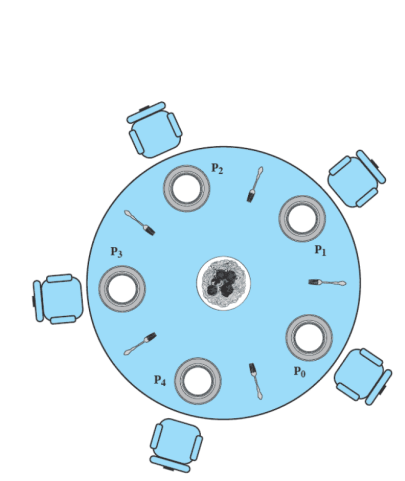
\includegraphics[width=0.4\linewidth]{images/filosofi-a-cena.PNG}
        %\captionof{figure}{Esempio di semaforo}
    \end{minipage}

    Ci sono due soluzioni possibili a questo problema. La prima utilizza i semafori:
    \begin{lstlisting}[language=C]
    semaphore fork[N] = {1 , 1 , ... 1};
    philosopher(int me) {
        int left, right, first, second;
        left = me;
        right = (me + 1) % N;
        first = right < left ? right : left;
        second = right < left ? left : right;
        while(1) {
            think();
            wait(fork[first]);
            wait(fork[second]);
            eat();
            signal(fork[first]);
            signal(fork[second]);
        }
    }
    \end{lstlisting}

    Una seconda soluzione utilizza i messaggi:
    \begin{lstlisting}[language=C]
    philosopher(int me) {
        int left, right;
        message fork1, fork2;
        left = me;
        right = (me + 1) % N;
        while(1) {
            think_for_a_random_time();
            if(nbreceive(fork[left], fork1)) {
                if(nbreceive(fork[right], fork2)) {
                    eat();
                    nbsend(fork[left], fork2);
                }
                nbsend(fork[right], fork1);
            }
        }
    }
    \end{lstlisting}
\end{Example}

\section{Deadlock e Linux}
In Linux, come sempre, si ha gestione minimale ma il più possibile efficiente. Quindi se dei processi utente sono scritti male e vanno in deadlock allora saranno tutti bloccati e sta all'utente accorgersene e killarli. Per quanto riguarda il kernel, c'è la prevenzione
dell'attesa circolare.